% !!!!!!!!!!!!!!!!!!!!!!!!!!!!!!!!!!!!!!!!!!!!!!!!!!!!!!!!!!!!!!!!!!!!!!!!!!!!
%                                                                            !
% Adapt this file so that you can use it for your thesis					 !
%                                                                            !
% !!!!!!!!!!!!!!!!!!!!!!!!!!!!!!!!!!!!!!!!!!!!!!!!!!!!!!!!!!!!!!!!!!!!!!!!!!!!


\documentclass{micro-econ-thesis}
\usepackage{graphicx}
\usepackage{setspace}
\usepackage{float}
\usepackage[utf8]{inputenc} % depends on the font encoding that you are using

% For formatting of your bibliography, please use the following package with options 
\usepackage[style=authoryear]{biblatex}
\usepackage{gensymb}

\addbibresource{bibliography.bib} % add a bib-reference file

\begin{document}
% ----------------------------------------------------------------------------
% Details for the titlepage
% ----------------------------------------------------------------------------
\thesisTitle{Develeopment of Analysis Techniques for dynamic magnetic resonance imaging}
\thesisType{Master Thesis} % 'Master Thesis' or 'Seminar Paper'
\thesisAuthor{Aayush Nepal}
\thesisMail{aayush.nepal@uni-jena.de}
\thesisGrade{Master of Science in Medical Photonics} % leave empty for seminar papers
\thesisTutora{Prof. Dr. rer. nat. med. habil. Jürgen Reichenbach}
\thesisTutorb{Dr. rer. nat. Martin Krämer}
\thesisMatrikel{198683}
\thesisAddress{Schützenggase 2\\[.5ex]
								99423 Weimar}
\thesisDate{\today}
% In case of external supervisor
\thesisCompany{}

% Print titlepage
\thesisMakeTitle

% ----------------------------------------------------------------------------
% Abstract
% ----------------------------------------------------------------------------
\cleardoublepage
\pagenumbering{roman}
\pagestyle{plain}
%\thispagestyle{empty}
\subsection*{Abstract}
Short summary of your thesis (max. 250 words) \ldots

\clearpage
\subsection*{Acknowledgements}
If you want to thank anyone (optional) \ldots

% ----------------------------------------------------------------------------
% Table of contents
% ----------------------------------------------------------------------------
\cleardoublepage
%\thispagestyle{empty}
\tableofcontents

% ----------------------------------------------------------------------------
% List of figures/tables
% ----------------------------------------------------------------------------
\cleardoublepage
\phantomsection
\addcontentsline{toc}{section}{List of Figures}
\listoffigures
% --------------------------
\cleardoublepage
\phantomsection
\addcontentsline{toc}{section}{List of Tables}
\listoftables
% --------------------------

\cleardoublepage
\phantomsection
\addcontentsline{toc}{section}{List of Acronyms}
\section*{List of Acronyms}
\begin{tabular}{@{}ll}
FSU Jena & Friedrich-Schiller-Universität Jena\\
\end{tabular}

% --------------------------

% ----------------------------------------------------------------------------
% Contents
% ----------------------------------------------------------------------------
\cleardoublepage
\pagestyle{headings}
\pagenumbering{arabic}
\setcounter{page}{1}
% Contents
\onehalfspacing % for linespacing 1.5, you can turn it off with \singlespacing, e.g. for quotes or tables with multiline cells


\section{Introduction}
\label{sec:intro}


\subsection{The Knee }
The knee, a pivotal structure in the human body, plays an essential role in locomotion, supporting not just the physical weight of the individual but also facilitating a wide range of movements crucial for daily activities. Beyond its mechanical functions, the knee's health and integrity are vital for overall quality of life, influencing everything from basic mobility to participation in complex sports. In a comprehensive survey across 15 European countries and Israel, it was found that knee pain was the third most commonly reported location of chronic pain, highlighting the significant concern it poses to public health \parencite{breivik_survey_2006}. Furthermore, arthritis/osteoarthritis (OA) was identified as the most common cause of this pain. 

And this situation has not improved with time. In Germany, a recent retrospective study has found that the number of patients with OA is steadily rising \parencite{obermuller_epidemiology_2024}. 
Part of the reason knee-related issues are so prevalent and impactful is the inherent complexity of the knee joint itself. As a hub of various anatomical structures working in unison, the knee supports a range of movements and bears significant loads, making it susceptible to a variety of injuries and conditions.
Understanding the anatomy of the knee is the first step in tackling this problem. 

\textbf{Anatomy and Function}

The knee joint is the largest and the most superficial joint. (cite Moore's clinically oriented anatomy page 1203, 9th ed wolters kluwer) 
The knee joint is the largest synovial joint in the body. (susan 2016, 1383 ) 
The knee joint consists of three articulations in one: one between each condyle of the femur and the corresponding tuberosity of the tibia, which are condyloid joints, and one between the patella and the femur. (cite anatomy descriptive and surgical 15th ed barnes and noble)
The knee joint is mechanically relatively weak because of the configurations of its aritcular surfaces. (cite Moore's clinically oriented anatomy 2nd edition). 
\begin{figure}[H]
	\centering
	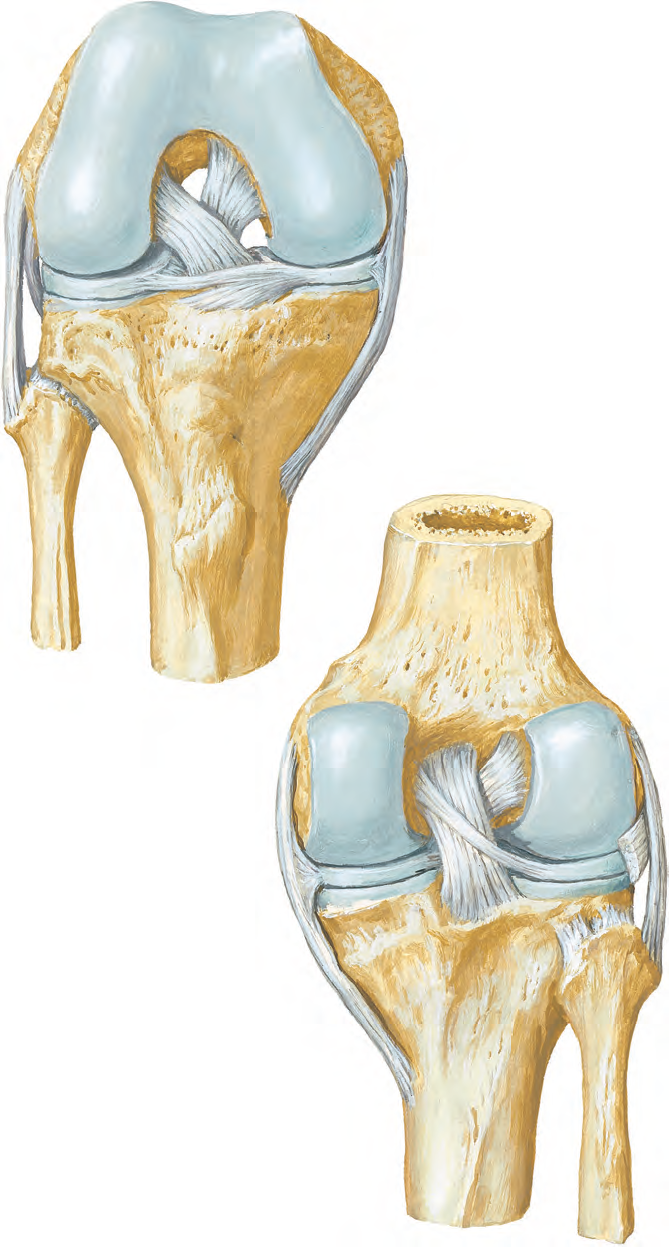
\includegraphics[width=0.7\linewidth]{right_knee_plate_519}
	\caption{Anterio and posterior view of the right knee, with the articular surfaces labelled \parencite{netter_519_2023}}
	\label{fig:rightkneeplate519}
\end{figure}


Importance of Imaging for Knee Analysis:

Directly link the discussion on anatomy and function to the utility of imaging, specifically MRI, highlighting how detailed knee structure and motion understanding is crucial for accurate imaging.
Introduce the concept of dynamic MRI here as a method that offers enhanced capabilities to observe and analyze the knee's dynamic nature, bridging directly to the next section without a separate transition.
\subsection{Dynamic MRI}
Begin this section by highlighting the limitations of traditional MRI in capturing the full range of knee joint motion, setting the stage for the introduction of dynamic MRI.
Outline the importance of dynamic MRI in knee analysis, emphasizing how it provides a more nuanced and complete picture of knee mechanics, especially in motion.
Discuss the applications of dynamic MRI in biomechanics and review existing methods for analyzing dynamic knee MRI data, setting the context for your research.

\subsection{Foundational Work}
Describe the two key papers that form the foundation of your thesis: the construction of the MRI knee loading device \parencite{brisson_novel_2022} and the development of the imaging sequence used for capturing data. \parencite{aleksiev_high-resolution_2022}

\subsection{Research Necessity}
Discuss the necessity for further analysis of the acquired images, emphasizing the gap between data collection and data interpretation within the current literature.

Clearly state the objectives of your research, focusing on the development of new analytical techniques to interpret the existing dynamic MRI data.

Explain the expected contributions of your research to the field, including the potential implications for biomechanical understanding and clinical applications.

\subsection{Thesis Structure}
Structure of the thesis is as follows: 


\section{Methodology}
\label{sec:second}
some text 
\subsection{Data Collection Methods}
\subsubsection{The Device}
A novel MRI-compatible device was integrated into the MRI scanner setup to facilitate guided knee motion in patients \parencite{brisson_novel_2022}. This device allowed for a range of motion of approximately 30 degrees, enabling subjects to perform knee flexion and extension cycles under both loaded and unloaded conditions. For loading, the device was equipped with compartments for weight plates \underline{(maybe picture here?)} and sandbags, providing a physiological load of 10 to 12 kilograms. 


Central to this device's functionality is an optical fiber position sensor \underline{actual citation needed?}(MR338-Y10C10, Micronor, 155 Camarillo, CA, USA), which precisely  which measures the ab­
solute angle from 0{\degree}\,to 360\degree \, with a resolution of 0.025\degree. This measurement capability is critical for synchronizing the knee's movement with MRI data reconstruction. To enhance signal acquisition and the clarity of imaging, two flexible coils \underline{(cite the coils here, perhaps also show a picture)} were positioned at key anatomical locations: one at the distal femur and another at the proximal tibia, as specified in the MRI protocol. \underline{perhaps show a picture outside the scanner of the patient wearing it? }

\subsubsection{Procedure Details}
***MRI measurements were performed on four healthy volunteers (aged between 28 and 37 years, body mass between 55 and 90 kg) using a clinical 3 T Siemens Prisma fit scanner. Volunteers had no known musculoskeletal conditions and gave written informed consent in accordance with the guidelines set out by the institutional ethics committee.*** \underline{from device paper} For all of these subjects, the left leg was used. 

The thigh is secured on a wedge positioner, and the lower leg is attached to an ankle rest, just above the malleoli, using Velcro straps to minimize lateral movement. Once positioned at the scanner's isocenter, the volunteer then engages in a controlled exercise, following a metronome set at 60 beats per minute. This pace dictates a four-beat flexion to extension cycle, where the leg is flexed at the first beat and fully extended by the fourth. This exercise is performed for approximately 2 minutes throughout the duration of the scan, totaling between 100 to 120 repetitions. Initially conducted under a loaded condition with weights, the process is repeated without the added resistance to compare both states.

\subsubsection{Sequence Parameters and Reconstruction}


\subsection{Data Analysis}
All the analysis and data visualization were done using the python programming language (v3.11.5). To begin, the data in nifti (Neuroimaging Informatics Technology Initiative) format is loaded using nibabel (v5.1.0) library. It is then visualized using napari(v0.4.18), a multi-dimensional interactive image viewer in Python. 
\subsubsection{Segmentation}
Step 1: Edge Detection Using the Canny Algorithm

The Canny filter \parencite{canny_computational_1986}, as implemented in the scikit-image's feature library (v0.21.0), was employed to apply an edge filter to the images. Various parameters of the Canny algorithm were adjusted, including edge thresholds and Gaussian blur, to optimize edge detection. Subsequently, the scikit-image's morphology library was utilized to remove small elements from the binary image. The image was then skeletonized to a one-pixel width, retaining only long and consistent edges. The final selection of the desired edge was accomplished using scipy's label algorithm (v1.11.3).

\subsection{Validity and Reliability}
Validation Methods: Detail the steps taken to validate the segmentation techniques and the biomechanical parameters you derived.
Reliability Measures: Describe any repeat analyses or cross-verifications done to ensure the consistency and reliability of your results.

\section{Results}
\label{sec:yetanother}

\subsection{Segmentation}
\label{subsec:last}
some text 

\subsection{Parameter Extraction}
some text 

\section{Discussion}
\subsection{Technique Evaluation}
Assess the effectiveness and accuracy of your segmentation techniques. 
\subsection{Biomechanical Insights}
Discuss the biomechanical parameters obtained and their implications for understanding knee movement. 
\subsection{Comparison with Existing Methods}
Compare your results with current analysis techniques. 
 

\section{Conclusion}
\subsection{Summary of Contributions}
Recap the novel analysis techniques developed and their significance. 
\subsection{Limitations and Challenges}
Discuss any limitations encountered and the challenges in the analysis process 
\subsection{Future Work}
Suggest potential improvements and future directions for research

% ----------------------------------------------------------------------------
% Bibliography
% ----------------------------------------------------------------------------
\cleardoublepage
\phantomsection
\addcontentsline{toc}{section}{\refname} % to add Bibliography to toc
\printbibliography

% --------------------------
\cleardoublepage
\begin{appendix}
\section{Appendix}
If needed for supplementary material, such as detailed description of data collection, tables, or figures.

\end{appendix}

% ----------------------------------------------------------------------------
% Statutory declaration
% ----------------------------------------------------------------------------
\makeThesisDeclaration

\end{document}

